\chapter{Εκτέλεση εργασίας και επαλήθευση}
\InitialCharacter{Τ} ο στάδιο εκτέλεσης και επαλήθευσης της εργασίας αποτελεί τον πυρήνα της αποκεντρωμένης εφαρμογής (\en{dApp}), διασφαλίζοντας ότι οι υπολογιστικές εργασίες όχι μόνο εκτελούνται με ακρίβεια και αποτελεσματικότητα από τον επιλεγμένο πάροχο, αλλά και ότι τα αποτελέσματα είναι επαληθεύσιμα και γνήσια. Αυτό το κεφάλαιο εμβαθύνει στις ιδιαιτερότητες της εκτέλεσης εργασιών, στον μηχανισμό που χρησιμοποιείται για την επαλήθευση της ορθότητας της εκτέλεσης και στην ασφαλή και διαφανή διαδικασία πληρωμής που διευκολύνεται από την τεχνολογία \en{Blockchain}.


\section{Εκτέλεση εργασιών}
Η εκτέλεση μιας υπολογιστικής εργασίας είναι μια σχολαστική διαδικασία, η οποία διασφαλίζει ότι ο πάροχος τηρεί τις προκαθορισμένες απαιτήσεις και εκτελεί την εργασία εντός του καθορισμένου περιβάλλοντος.
\begin{enumerate}
    \item Ενεργοποίηση της εργασίας: Μετά την επιλογή του από τον πελάτη, ο πάροχος ενεργοποιεί την εργασία, σηματοδοτώντας τη δέσμευσή του για την εκτέλεσή της. Στα πλαίσια της δέσμευσης αυτής, στο σημείο αυτό στέλνει στο συμβόλαιο χρηματική εγγύηση ίση με την αξία εκτέλεσης της εργασίας για 2 δευτερόλεπτα.
    \item Περιβάλλον απομόνωσης: Για να διασφαλιστεί το σύστημα του παρόχου και να εξασφαλιστεί ένα συνεπές περιβάλλον εκτέλεσης, οι εργασίες εκτελούνται εντός \en{Docker container}. Αυτή η ενθυλάκωση απομονώνει την εκτέλεση από εξωτερικές παρεμβάσεις και πιθανές απειλές ασφαλείας.
    \item Ανάκτηση κώδικα: Ο πάροχος ανακτά τη μεταγλωττισμένη κλάση \en{Java} του πελάτη από το \en{IPFS} χρησιμοποιώντας το \en{CID} της.
    \item Εκτέλεση εργασιών: Εντός του \en{Docker container}, η κλάση \en{Java} εκτελείται, τηρώντας τη λογική που περιέχεται στη μέθοδο \textit{\en{getComputation}} από τον πελάτη.
    \item Αποστολή αποτελεσμάτων: Τα αποτελέσματα εκτέλεσης της υπολογιστικής εργασίας αποθηκεύονται σε ένα αρχείο, μεταφορτώνονται στο \en{IPFS} και το \en{CID} τους αποστέλλεται στο \en{smart contract} ώστε να το λάβει ο πελάτης μετά την ολοκλήρωση της πληρωμής του.
\end{enumerate}

\section{Μηχανισμός επαλήθευσης}
Η διασφάλιση της πραγματικής εκτέλεσης της εργασίας είναι καθοριστικής σημασίας και η \en{dApp} χρησιμοποιεί έναν ισχυρό μηχανισμό επαλήθευσης για να εξακριβώσει τη γνησιότητα των αποτελεσμάτων.

\begin{enumerate}
    \item Συμβολοσειρά επαλήθευσης: Η μέθοδος \textit{\en{getVerification}} εντός της εκτελούμενης κλάσης \en{Java} επιστρέφει μια προκαθορισμένη συμβολοσειρά, η οποία είναι άγνωστη στον πάροχο.
    \item Σύγκριση κατακερματισμένης συμβολοσειράς: Η επιστρεφόμενη συμβολοσειρά επαλήθευσης κατακερματίζεται και συγκρίνεται με τον αρχικό κατακερματισμό που δόθηκε από τον πελάτη κατά την έναρξη της δημοπρασίας.
    \item Επικύρωση αποτελέσματος: Εάν οι κατακερματισμένες συμβολοσειρές ταιριάζουν, το αποτέλεσμα θεωρείται γνήσιο και η εργασία κρίνεται επιτυχημένη.
    Αντίθετα, μια αναντιστοιχία υποδηλώνει ασυμφωνία, ενεργοποιώντας την ανεπιτυχή ροή της εργασίας.
    \item Επαλήθευση χρόνου: Επιπλέον, ο χρόνος εκτέλεσης επαληθεύεται σε σχέση με τη συμφωνηθείσα προθεσμία, ώστε να διασφαλιστεί η έγκαιρη ολοκλήρωση της εργασίας.
\end{enumerate}

\section{Διαδικασία πληρωμής}
Μετά την επιτυχή επαλήθευση, ξεκινά η διαδικασία πληρωμής, διασφαλίζοντας μια διαφανή συναλλαγή μεταξύ του πελάτη και του παρόχου.

\begin{enumerate}
    \item Υπολογισμός πληρωμής: Το ποσό πληρωμής υπολογίζεται με βάση τη συμφωνηθείσα τιμή (\en{wei} ανά δευτερόλεπτο) και τον πραγματικό χρόνο εκτέλεσης. Από αυτό αφαιρείται το ποσό που έχει ήδη στείλει στο συμβόλαιο ο πελάτης ως χρηματική εγγύηση.
    \item Συναλλαγή \en{blockchain}: Η πληρωμή πραγματοποιείται μέσω του έξυπνου συμβολαίου \en{TasksManager} στο \en{Ethereum  blockchain}, εξασφαλίζοντας ασφάλεια και διαφάνεια.
    \item Χειρισμός εγγυήσεων: Μετά την επιτυχή εκτέλεση της εργασίας, επιστρέφονται στον πάροχο οι χρηματικές εγγυήσεις που είχε αποστείλει κατά την έναρξη της διαδικασίας. Σε περιπτώσεις ανεπιτυχούς εκτέλεσης της εργασίας, οι χρηματικές εγγυήσεις του υπεύθυνου χάνονται, όπως περιγράφεται λεπτομερώς στο προηγούμενο κεφάλαιο.
\end{enumerate}

Παρακάτω παρουσιάζεται ο κύκλος ζωής μιας εργασίας (\en{Task}), με βάση τις καταστάσεις \en{TaskState} και \en{PaymentState} της οντότητας \en{Task}.
\begin{illustration}
    \centering
    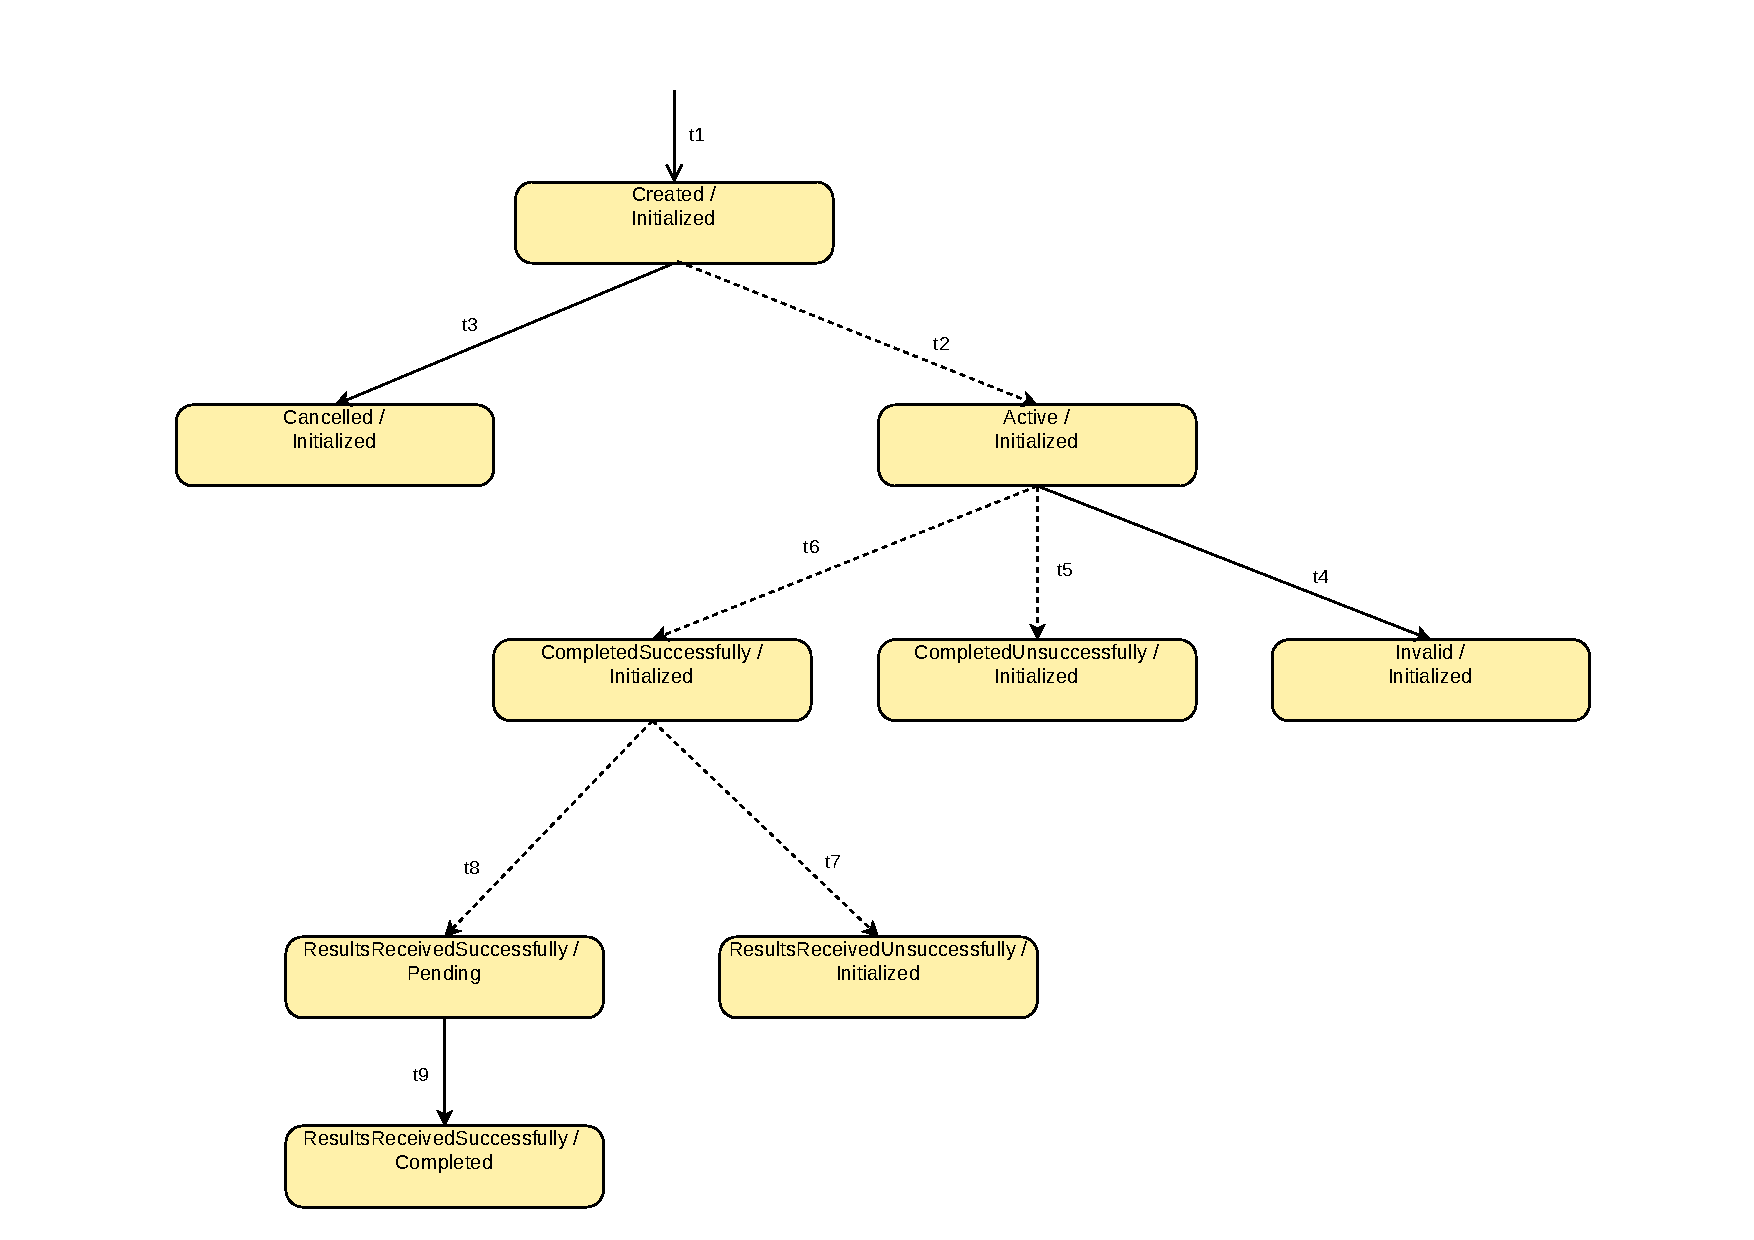
\includegraphics[width=1.2\textwidth]{figures/figure-007.pdf}
    \caption{\en{State machine} του \en{Task}, με βάση το \en{TaskState/PaymentState}}
    \begin{minipage}{\textwidth}
        \small
        \text{Η μετάβαση \en{t1} πραγματοποιείται από το \en{AuctionsManager} μετά από την αντίστοιχη ενέργεια του \en{client}.}
        \text{Οι μεταβάσεις \en{t3, t4} και \en{t9} πραγματοποιούνται από τον \en{client}}, ενώ οι μεταβάσεις \en{t2, t5, t6, t7, t8} και \en{t10}  από τον \en{provider}.
      \end{minipage}
\end{illustration}


\newpage
\section{Ασφάλεια κατά την εκτέλεση και την πληρωμή}
Η \en{dApp} διακατέχεται από διάφορα μέτρα ασφαλείας για τη διασφάλιση των συμφερόντων τόσο των πελατών όσο και των παρόχων κατά την εκτέλεση και την πληρωμή.
\begin{itemize}
    \item[-] Αμετάβλητες λεπτομέρειες εργασιών: Οι λεπτομέρειες των εργασιών, αφού μεταφορτωθούν στο \en{IPFS}, είναι αμετάβλητες, διασφαλίζοντας ότι η εκτέλεση τηρεί τις αρχικές απαιτήσεις.
    \item[-] Απομονωμένο περιβάλλον εκτέλεσης: Το \en{Docker container} διασφαλίζει ότι το σύστημα του παρόχου παραμένει απομονωμένο από πιθανό κακόβουλο κώδικα και ότι το περιβάλλον εκτέλεσης είναι συνεπές. 
    \item[-] Διαφανείς συναλλαγές: Όλες οι συναλλαγές, συμπεριλαμβανομένων των πληρωμών και των τοποθετήσεων εγγυήσεων, καταγράφονται στο \en{blockchain}, εξασφαλίζοντας διαφάνεια και επαληθευσιμότητα.
    \item[-] Μηχανισμός εγγυήσεων:  Ο μηχανισμός εγγυήσεων διασφαλίζει τη δέσμευση και των δύο μερών και χρησιμεύει ως αποτρεπτικός παράγοντας έναντι κακόβουλων δραστηριοτήτων ή μη συμμόρφωσης.
\end{itemize}


Ανακεφαλαιώνοντας, το στάδιο εκτέλεσης και επαλήθευσης των εργασιών είναι σχολαστικά σχεδιασμένο ώστε να διασφαλίζεται ότι οι εργασίες εκτελούνται με ακρίβεια, τα αποτελέσματα είναι επαληθεύσιμα και οι πληρωμές είναι ασφαλείς και διαφανείς. Αυτή η φάση, η οποία υποστηρίζεται από την τεχνολογία \en{blockchain} και τους μηχανισμούς που περιγράφηκαν, ενισχύει την αξιοπιστία της \en{dApp} στο αποκεντρωμένο υπολογιστικό νέφος.
